
\section{Creating Maven project from the archetype}

For this homework, we create another archetype called
\texttt{hellobioqa-archetype} to help you quickly get your development started.
We briefly show you the process you've gone through for your Homework 1.

\begin{enumerate}

\item Open your Eclipse's \textbf{Preferences} window, and navigate to
\textbf{Maven} $\rightarrow$ \textbf{Archetypes}, and click \textbf{Add Remote
Catalog\ldots}.

\item Type the following URL into the \textbf{Catalog File} field.

\small
\begin{verbatim}
http://ziy.github.com/hellobioqa-archetype/repository/archetype-catalog.xml
\end{verbatim}
\normalsize

Optionally, you can add a \textbf{Description} for this catalog, for example
``HelloBioQA Catalog''. Then click \textbf{OK} on the \textbf{Remote Archetype
Catalog} window and another \textbf{OK} on the \textbf{Preferences} window.

\item Include the following lines in your \texttt{settings.xml} in order to
download the artifact if you didn't do so in Homework 1.

\lstinputlisting[language=XML,float,linewidth=1.1\textwidth,caption=Configuring settings.xml,label=settings]{settings.xml}

\item Now you can follow almost the same steps to import to Eclipse as you did
for Homework 1. Since we have created the archetype for you, remember to
unselect \textbf{Create a simple project (skip archetype selction)}. Then click
\textbf{Next}.
 
\item Here you can select ``HelloBioQA Catalog'' (or other names you specified
in the previous step) or ``All Catalogs'' in the drop-down menu for
\textbf{Catalog}. Then, type in ``hellobioqa-archetype'' (without quotes) in the \textbf{Filter}
field, and in order to get the latest snapshot archetypes, you need to check
\textbf{Include snapshot archetypes} as well. Select the archetype listed below,
and click next to continue.

\item In the next window, you are asked to specify the \textbf{Group Id} and
\textbf{Artifact Id}. Similar to Homework 0 and 1, the Group Id is

\begin{center}
\textbf{edu.cmu.lti.11791.f12.hw2}
\end{center}

and Artifact Id is

\begin{center}
\textbf{hw2-teamXX}
\end{center}

with XX being your team number. Since we also included two sample components for
retrieval strategist and passage extraction within a particular, remember to
specify \texttt{Package} as

\begin{center}
\textbf{edu.cmu.lti.oaqa.openqa.hellobioqa}
\end{center}

See Figure \ref{fig:package-name}. Then click \textbf{Finish}.

\begin{figure}[t]
\centering
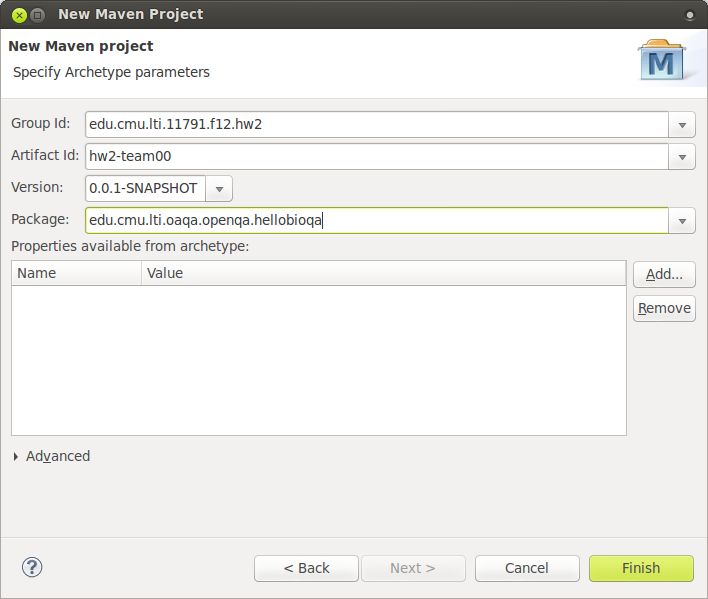
\includegraphics[scale=0.3]{package-name}
\caption{Parameters to create a Maven artifact from archetype\label{fig:package-name}}
\end{figure}

\item You need to edit the \texttt{pom.xml} file to type in the SCM information
of your GitHub repository for Homework 2 as you did in Homework 0.

\item You also need to manually edit the \texttt{launches/hellobioqa.launch}
file. Open the file, replace the \verb|${project_name}| with your project name
(e.g., \verb|hw2-team00|).

\item Same as before, you probably need to right-click the project name, and
click \textbf{Maven} $\rightarrow$ \textbf{Update Project} to download the
dependencies.

\end{enumerate}

You can see that we have included

\begin{itemize}

\item the \texttt{pom.xml}. You can go to the \textbf{Dependencies} tab after
you double-click the pom file, and you will be able to see your project only
depends on \texttt{helloqa} project, which brings simple implementations for all
the phases described in \texttt{baseqa} project. You won't need any direct
dependency on any UIMA SDK package, which are essential to your Homework 1.

If you want to take a look at what are inside \texttt{helloqa} project and
other indirect dependencies, you can unfold the \texttt{Maven Dependencies}
folder under your project name in the Package Explorer View.

\item input file in the \texttt{src/main/resources/input} folder, and
gold-standard annotations in the \texttt{src/main/resources/gs} folder. If you
are interested in their contents, you can open them with a text editor.

\item several descriptors under \texttt{src/main/resources/hellobioqa} directory
and subdirectories. All of them are specific to the hellobioqa task, and
actually, you can find more descriptors from dependencies, e.g.,
\texttt{helloqa}, \texttt{jdbc-provider}, etc. These descriptors can also be
considered to incorporate in your project.

\item the main yaml \texttt{src/main/resources/hellobioqa/hellobioqa.yaml}

\item an Eclipse launch file \texttt{launches/hellobioqa.launch}. To run the
pipeline, you can right-click this file in the Package Explorer View, and then
click \textbf{Run As} $\rightarrow$ \textbf{hellobioqa}.

\item a local database version of the cse repository
\texttt{data/oaqa-eval.db3}. All your experiment intermediate result and
evaluation results will be permanently stored here (unless you manually delete
table entries), and you will find the file may grow to several megabytes after
thundreds of experiments. Therefore, we suggest you should not commit this file
to the GitHub repository, instead you can \texttt{git ignore} this file to avoid
this huge file bothering you every time you commit your project.

\end{itemize}

Before you commit and push all the initial code changes to GitHub repository, we
suggest you to first test if you can successfully run the pipeline.

\begin{enumerate}

\item Right-click this file in the Package Explorer View, and then click
\textbf{Run As} $\rightarrow$ \textbf{hellobioqa}. Wait until all 28 questions
are processed, and the evaluation results are printed to the console, and you
find no exceptions are thrown.

\item Git-ignore \texttt{data/oaqa-eval.db3}\footnote{Since your team member
also needs the database file to run experiment, the team leader can add it to
the index first then remove it after team members clone the project to their
machines, or all the members can download an empty file from here:
\url{https://github.com/oaqa/helloqa/blob/a051e1233be92bca309ff8761835fce412f6bfd5/data/oaqa-eval.db3?raw=true},
and put it under \texttt{data/}.}, and commit/push all other code changes to the
GitHub repository. Remember to commit the .project file, .classpath file and all
other important configuration files from your project root directory, and it
will be helpful for your team members to directly import an existing project.

\item Now, other team members are able to clone the repository to their
workspaces and start working on particular task. When you are asked to
\textbf{Select a wizard to use for importing projects}, don't forget to select
\textbf{Import existing projects} as long as your team leader commited .project
and .classth to the repository.

\end{enumerate}
